%--------
% Notes:
%   ~ADD       : Add the following.
%   ~REFERENCE : Reference the following paper/authors.
%   ~FIND      : Find a paper regarding the following.
%   ~CHECK     : Check that the following is met.
%   ~READ      : Read through the following paper/authors.
%   ~MENTION   : Mention the following.
%   ~AMMEND    : Make a change to the following.
%   ~IDEA      : Suggestion for later in the project.

\documentclass{UoYCSproject}
% Tikz Setup
\usepackage{tikz}
\usetikzlibrary{ matrix,      % For easy node positioning
                 fit,         % For easily fitting nodes inside another one
                 arrows,
                 positioning, % For easy node-relative placements
               }
\tikzstyle{edge} = [->, bend left]
\tikzstyle{vertex} = [circle, minimum width=0.5cm, text centered, draw=black]
\tikzstyle{graph} = [rectangle, draw=black, inner sep=1cm]
\tikzstyle{rule} = [rectangle, inner sep=1cm]
\tikzstyle{derivation} = [-implies, double]
% Listings Setup
\usepackage{listings}
\renewcommand{\lstlistingname}{C Code}

\author{Huw Taylor}
\title{Tracing and Debugging GP2}
\date{\today}
\supervisor{Dr. Detlef Plump}
\MEng
\wordcount
% ~CHECK: The bibTex reference LaTeX word count has the `accessed` field updated.
% ~16000 words (55 pages) total
\pagecount
\abstract{
% ~66 words
}
\acknowledgements{

}

\begin{document}

\maketitle
\tableofcontents
\listoffigures

\chapter{Introduction}
% ~1333 words
\section{Motivation}
The University of York has produced a graphical editor for creating graphs and graph programs. The editor depends on a compiler to produce the resultant graph, also made at the University of York. Both these tools are planned to be used by students in the coming academic year (2016/2017) for the GRAT module taught there.
The aim of this project is to show the intermediate steps of the programme, so that correctness of the compiler and the graphical editor can be ensured, and also so that students using these tools, learning how graph programs work, can see the process with a finer granularity.
\section{Ethics}
The project discussed has very few ethical considerations. It is not related to defence and there are no safety or security concerns.

\chapter{Literature Review}
% ~4000 words
% ~CHECK: Shows that you know what is happening in your field 
% ~CHECK: Justifies why your work is interesting or important 
% ~CHECK: establishes the theoretical framework/context for your work 
% ~CHECK: defends your choice of methodology 
% ~CHECK: avoids repeating previous researchers’ mistakes
\section{Graph Programming}
\subsection{Graph Transformations}
A graph is a visual way of representing data and relationships. The formal definition is a set of vertices (nodes) \emph{V}, a set of edges \emph{E}, and a set of labels \emph{L}. Additionally \emph{source} and \emph{target} functions associate edges with nodes, and a \emph{label} function, which assigns labels to edges and nodes.
This field was first proposed in the 1970s by Ehrig, Pfender \& Schneider \cite{grat_origin}.
\emph{TO~ADD: briefly mention double-pushout/single-pushout methods and give graphical examples.} % ~ADD: references to double-pushout and single-pushout methods, as well as contributions to graph theory in general
The mathematical theory of Graph Transformation allows the transformation of graphs by way of rules. Rules are applied to graphs. They include a LHS (Left-Hand Side) graph, and RHS (Right-Hand Side) graph and an interface graph, which connects nodes in the LHS to nodes in the RHS. There is a convention that if the interface graph is ommited then it is inferred that it comprises the common labelled nodes in both the LHS and RHS.

Figure \ref{fig:simple_rule} on page \pageref{fig:simple_rule} shows a simple rule that creates a transative graph, where every node accessible by another has a direct edge going to it. Figure \ref{fig:simple_rule_sans_k} on page \pageref{fig:simple_rule_sans_k} shows the same rule without its interface graph.

\begin{figure}
\label{fig:simple_rule}
\centering
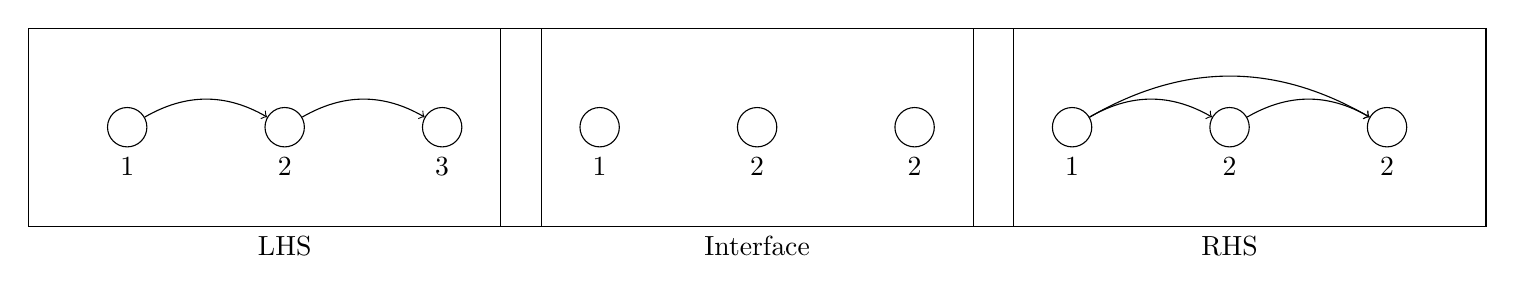
\begin{tikzpicture}[scale=2]
  \node (n1) [vertex, label=below:{1}] at (0, 0) {};
  \node (n2) [vertex, label=below:{2}] at (1, 0) {};
  \node (n3) [vertex, label=below:{3}] at (2, 0) {};
  \path [edge] (n1) edge node {} (n2);
  \path [edge] (n2) edge node {} (n3);
  \node (l) [graph, fit={(n1) (n2) (n3)}, label=below:{LHS}] {};
  
  \node (n4) [vertex, label=below:{1}] at (3, 0) {};
  \node (n5) [vertex, label=below:{2}] at (4, 0) {};
  \node (n6) [vertex, label=below:{2}] at (5, 0) {};
  \node (k) [graph, fit={(n4) (n5) (n6)}, label=below:{Interface}] {};
  
  \node (n7) [vertex, label=below:{1}] at (6, 0) {};
  \node (n8) [vertex, label=below:{2}] at (7, 0) {};
  \node (n9) [vertex, label=below:{2}] at (8, 0) {};
  \path [edge] (n7) edge node {} (n8);
  \path [edge] (n8) edge node {} (n9);
  \path [edge] (n7) edge node {} (n9);
  \node (r) [graph, fit={(n7) (n8) (n9)}, label=below:{RHS}] {};
\end{tikzpicture}
\caption{Rule Example}
\end{figure}

\begin{figure}
\label{fig:simple_rule_sans_k}
\centering
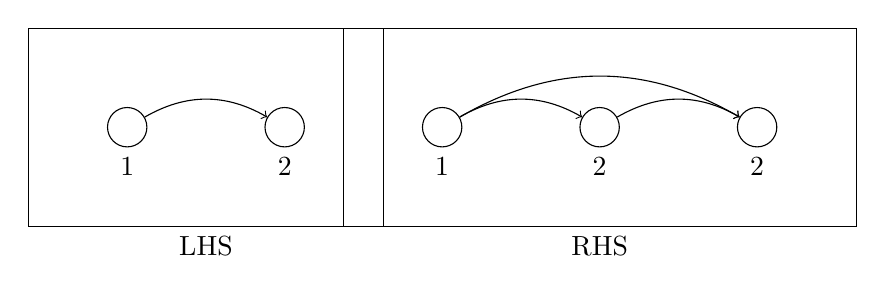
\begin{tikzpicture}[scale=2]
  \node (n1) [vertex, label=below:{1}] at (0, 0) {};
  \node (n2) [vertex, label=below:{2}] at (1, 0) {};
  \path [edge] (n1) edge node {} (n2);
  \node (l) [graph, fit={(n1) (n2)}, label=below:{LHS}] {};
  
  \node (n7) [vertex, label=below:{1}] at (2, 0) {};
  \node (n8) [vertex, label=below:{2}] at (3, 0) {};
  \node (n9) [vertex, label=below:{2}] at (4, 0) {};
  \path [edge] (n7) edge node {} (n8);
  \path [edge] (n8) edge node {} (n9);
  \path [edge] (n7) edge node {} (n9);
  \node (r) [graph, fit={(n7) (n8) (n9)}, label=below:{RHS}] {};
\end{tikzpicture}
\caption{Rule Example without Interface Graph}
\end{figure}

% ~READ, ~ADD: https://www.cs.york.ac.uk/plasma/wiki/index.php?title=GP_%28Graph_Programs%29 Lots of relevant papers and a couple of example programs i can steal and reference.
\subsection{Graph Programs}
The University of York has developed a graph programming language \emph{GP} \cite{gp1}, and has developed a new implementation \emph{GP2}. The goal of both of these has been to write programs that manipulate graphs in terms of the graphs, rather than in general purpose languages like C or Java. The first GP was produced by Greg Manning. % ~ADD, ~REFERENCE: Greg Manning Paper
GP allows the application of \emph{programs} to graphs. A program is made up of rules and rudimentary control structures, such as conditions, and loops. The rules are executed non-deterministically on a graph, known as the \emph{Host Graph}. The resulting graph is known as the \emph{Result Graph}. A simple program could just be the continued application of a single rule.

\begin{figure}
\label{fig:simple_program}
\centering
% ~ADD: Make the code portion of this picture truetype
% ~CHECK: Make sure this displays how it should (https://www.cs.york.ac.uk/plasma/wiki/images/5/5c/ExampleGraphProgramSimple_Dijkstra.png)
\begin{tikzpicture}[scale=2]
  \node (code) at (0, 1.5) {$main = InitTags!; Reduce$};
  \node (rule_1) at (0, 1) {$InitTags(a,b,c,n : int) = $};

  \node (n1) [vertex, label=below:{1}] at (0, 0) {a_n};
  \node (n2) [vertex, label=below:{2}] at (1, 0) {c};
  \path [edge] (n1) edge node[label=above:{b}] {} (n2);
  \node (r1_l) [rule, fit={(n1) (n2)}] {};
  
  \node (n3) [vertex, label=below:{1}] at (2, 0) {a_n};
  \node (n4) [vertex, label=below:{2}] at (3, 0) {c_n+b};
  \path [edge] (n3) edge node[label=above:{b}] {} (n4);
  \node (r1_r) [rule, fit={(n3) (n4)}] {};
  
  \draw[-implies,double, thick] (r1_l) -- (r1_r);
  
  \node (rule_2) at (0, 1) {$Reduce(a,b,c,n,i : int) = $};  
  
  \node (n5) [vertex, label=below:{1}] at (0, 1) {a_n};
  \node (n6) [vertex, label=below:{2}] at (1, 1) {c_i};
  \path [edge] (n5) edge node[label=above:{b}] {} (n6);
  \node (r2_l) [rule, fit={(n5) (n6)}] {};
  
  \node (n7) [vertex, label=below:{1}] at (2, 1) {a_n};
  \node (n8) [vertex, label=below:{2}] at (3, 1) {c_n+b};
  \path [edge] (n7) edge node[label=above:{b}] {} (n8);
  \node (r2_r) [rule, fit={(n7) (n8)}] {};
  
  \draw[-implies,double, thick] (r2_l) -- (r2_r);
  \node (rule_2_condition) at (0, 2) {$where n+b < i$};  

\end{tikzpicture}
\caption{Simple Dijkstra Program Example}
\end{figure}

The program \ref{fig:simple_program} on page \pageref{fig:simple_program} finds the shortest path to each node, using Dijkstra's algorithm for pathfinding. Running it on the host graph will give the intermediary graphs shown in \ref{fig:simple_program_example} on \pageref{fig:simple_program_example}. % ~ADD: Maybe break down the application of one rule. Show what's happening. Maybe somewhere else?

\begin{figure}
\label{fig:simple_program_example}
\centering
% ~CHECK: Make sure this displays how it should.
\begin{tikzpicture}[scale=2]
  \node (n1_1) [vertex] at (0, 0) {1_0};
  \node (n1_2) [vertex] at (1, 0) {2};
  \node (n1_3) [vertex] at (1, 1) {3};
  \node (n1_4) [vertex] at (1, 2) {4};
  \node (n1_5) [vertex] at (2, 1) {5};
  \path [edge] (n1_1) edge node[label=above:{4}] {} (n1_2);
  \path [edge] (n1_1) edge node[label=above:{6}] {} (n1_3);
  \path [edge] (n1_2) edge node[label=above:{1}] {} (n1_3);
  \path [edge] (n1_3) edge node[label=above:{2}] {} (n1_4);
  \path [edge] (n1_2) edge node[label=above:{6}] {} (n1_5);
  \path [edge] (n1_3) edge node[label=above:{4}] {} (n1_5);
  \path [edge] (n1_4) edge node[label=above:{1}] {} (n1_5);
  \node (g0) [rule, fit={(n1_1) (n1_2) (n1_3) (n1_4) (n1_5)}, label=below:{Host Graph}] {};
  
  \node (n2_1) [vertex] at (0, 0) {1_0}; % probably have to change these coordinates.
  \node (n2_2) [vertex] at (1, 0) {2_4};
  \node (n2_3) [vertex] at (1, 1) {3};
  \node (n2_4) [vertex] at (1, 2) {4};
  \node (n2_5) [vertex] at (2, 1) {5};
  \path [edge] (n2_1) edge node[label=above:{4}] {} (n2_2);
  \path [edge] (n2_1) edge node[label=above:{6}] {} (n2_3);
  \path [edge] (n2_2) edge node[label=above:{1}] {} (n2_3);
  \path [edge] (n2_3) edge node[label=above:{2}] {} (n2_4);
  \path [edge] (n2_2) edge node[label=above:{6}] {} (n2_5);
  \path [edge] (n2_3) edge node[label=above:{4}] {} (n2_5);
  \path [edge] (n2_4) edge node[label=above:{1}] {} (n2_5);
  \node (g1) [rule, fit={(n2_1) (n2_2) (n2_3) (n2_4) (n2_5)}, label=below:{Graph after one application of InitTags}] {};
  
  \node (n3_1) [vertex] at (0, 0) {1_0}; % probably have to change these coordinates.
  \node (n3_2) [vertex] at (1, 0) {2_4};
  \node (n3_3) [vertex] at (1, 1) {3_6};
  \node (n3_4) [vertex] at (1, 2) {4_8};
  \node (n3_5) [vertex] at (2, 1) {5_10};
  \path [edge] (n3_1) edge node[label=above:{4}] {} (n3_2);
  \path [edge] (n3_1) edge node[label=above:{6}] {} (n3_3);
  \path [edge] (n3_2) edge node[label=above:{1}] {} (n3_3);
  \path [edge] (n3_3) edge node[label=above:{2}] {} (n3_4);
  \path [edge] (n3_2) edge node[label=above:{6}] {} (n3_5);
  \path [edge] (n3_3) edge node[label=above:{4}] {} (n3_5);
  \path [edge] (n3_4) edge node[label=above:{1}] {} (n3_5);
  \node (gx) [rule, fit={(n3_1) (n3_2) (n3_3) (n3_4) (n3_5)}, label=below:{Graph after all possible applications of InitTags}] {}; 
  
  \node (n4_1) [vertex] at (0, 0) {1_0}; % probably have to change these coordinates.
  \node (n4_2) [vertex] at (1, 0) {2_4};
  \node (n4_3) [vertex] at (1, 1) {3_5};
  \node (n4_4) [vertex] at (1, 2) {4_7};
  \node (n4_5) [vertex] at (2, 1) {5_8};
  \path [edge] (n4_1) edge node[label=above:{4}] {} (n4_2);
  \path [edge] (n4_1) edge node[label=above:{6}] {} (n4_3);
  \path [edge] (n4_2) edge node[label=above:{1}] {} (n4_3);
  \path [edge] (n4_3) edge node[label=above:{2}] {} (n4_4);
  \path [edge] (n4_2) edge node[label=above:{6}] {} (n4_5);
  \path [edge] (n4_3) edge node[label=above:{4}] {} (n4_5);
  \path [edge] (n4_4) edge node[label=above:{1}] {} (n4_5);
  \node (gn) [rule, fit={(n4_1) (n4_2) (n4_3) (n4_4) (n4_5)}, label=below:{Graph after all possible applications of Reduce}] {}; 
  
\end{tikzpicture}
\caption{Simple Dijkstra Program Example}
\end{figure}

% ~ADD: first few iterations of this program on an example host graph.

GP2 has a number of differences in the way in which it was implemented. As well as trying to address the issues of maintainability and usability, several features were added.
Instead of using an abstract machine, GP2 generates C code directly \cite{chris_compiler}, which removes the reliance on YAM, the YAM compiler, and YAM graph and program formats. It means that any C compiler can be used to generate the bytecode. It also attempts to standardise and document the format of graphs and programs that it takes. This means that tools to generate graphs either graphically or programmatically can be created without reducing modularity or creating complexity and interdependance between the components of the system \cite{gp2_ide}.

GP2 no longer enforces non-detereministic execution \cite[p. 15]{gp2_ide}, and doesn't backtrack to reach all possible solutions. This was done to achieve a higher level of implementation efficiency \cite[p. 15]{chris_compiler}, but sacrifices completeness.
\emph{TO~ADD: mention the haskell interpreter but say it's not `official'.} % ~MENTION: no longer non-deterministic. no backtracking and no longer the case that all solutions will be reached. Maybe mention the haskel one and its optional backtracking.

\subsection{GP2 Editor}
The GP2 graphical editor for creating graphs and graph programs is currently under development. It will allow for the creation of graphs graphically, rather than textually, and it will allow for the creation of programs textually, and their rules graphically, assigning the LHS and RHS of the rules. In contrast with the GP1 editor, the GP2 editor will also include functionality to highlight nodes.

\section{Tracing and Debugging}
Tracing through the steps of a program has been around since programs themselves. % ~FIND: origins of tracing for debugging
It allows programmers to ensure that each step is procuding the right results and allows a more detailed insight into the workings of a program. This is done by logging information about the execution of a program that will be useful for debugging or diagnostics. 
Formal methods have been discussed as far back as the 70s \cite{psych_debug, code_walkthroughs}. 

% ~FIND: some papers on debugging
% ~READ: psych_debug and code_walkthroughs for stuff to say about tracing/debugging
% ~READ: https://bitbucket.org/pypy/extradoc/src/tip/talk/pepm2011/bolz-allocation-removal.pdf (reference #16 might be good)

% ~FIND, ~MENTION: a paper on TRON and mention it briefly.

% ~MENTION: tracing is a cross-cutting concern. It's difficult to decouple. It involves lots of the code.
% ~MENTION: due to tracing being low-level, the potential volume of logging is higher, which can have performace concerns. Usually this means the option of having it turned off at run- (or compile-) time, however because this is a feature of the editor, this is a bit awkward. 
% ~MENTION: Normally the tracing results are only really to be used be the developer and so don't need to be localised or presented in a particularly user-friendly way. However, this project the tracing is for students who don't know the graphs. So the tracing has to be presented in a way that's understandable.
% ~IDEA: Maybe have compile-time setting whereby *debugging* tracing can be turned off, but the *learning* tracing is still on. Or maybe have settings for both. debugging on/off. step production on/off. For performance reasons.

% END OF LITERATURE REVIEW

\chapter{Approach}
\section{Requirement Identification}
% ~2000 words
\begin{enumerate}
	\item Rules must be able to be stepped through one at a time.
 	\item The current rule must be made apparent graphically somehow.
	\item \ldots
\end{enumerate}
\section{Design}
% ~3333 words
\begin{itemize}
	\item Lifecycle
 	\item Engineering approach
 	\item Time management and/or general plan
	\item \ldots
\end{itemize}
 
\subsection{Tools}
Not a lot really.
\begin{itemize}
  \item Git
  \item Some C compiler/IDE/something or another
  \item Dependencies for GP-Editor
  \item \ldots
\end{itemize}
\section{Implementation}


\begin{lstlisting}[label=c_1, caption=Placeholder C Code]
*foo = &bar;
\end{lstlisting}


\chapter{Evaluation}
% ~3333 words
\chapter{Conclusions}
% ~1333 words
\section{Future Work}

% \bibliography{references}

\chapter{Appendices}
\end{document}